\documentclass[10pt]{beamer}

\usetheme{sthlm}

%%%% STHLM
\usepackage{metalogo}
%\usepackage[utf8]{inputenc}
\usepackage{%
	booktabs,
	datetime,
	dtklogos,
	pgfplots,
	ragged2e,
	tabularx,
	wasysym
}
\usepackage[scale=2]{ccicons}
%%%% /STHLM


\usepackage{nameref}
\makeatletter
\newcommand*{\currentname}{\currentlabelname}
\makeatother

\newcommand*{\footnotedef}[2]{#1\footnote{\textbf{#1}: #2}}
\newcommand*{\TODO}{{\color{red}TODO}}
\usepackage{xcolor}

\hypersetup{%
	colorlinks,
	linkcolor=sthlmBlue,
	urlcolor=sthlmBlue,
	linkbordercolor=sthlmBlue,
	pdfborderstyle={/S/U/W 1}
%	linkcolor={red!50!black}
	%linkcolor={196!0!100},
}

% so we don't have 'Figure x.x' on captions
\setbeamertemplate{caption}{\raggedright\insertcaption\par}

\title{An Introduction to Git}
\subtitle{Version Control for the Greater Good}
\date{\today}
\author{Jamie Tanna, \url{http://jvt.me}}
\institute{\href{http://hacksocnotts.co.uk}{Hacksoc Nottingham}
}

\begin{document}

\maketitle

\begin{frame}
	\frametitle{Overview}
	\setbeamertemplate{section in toc}[sections numbered]
	\tableofcontents
	% \tableofcontents[hideallsubsections]
\end{frame}

\section{An Introduction to Git}

\begin{frame}
	\frametitle{A Few Notes}

	\begin{alertblock}{git vs github}
		\href{http://www.git-scm.com/}{Git} $!==$ \href{https://github.com}{Github}
			\begin{itemize}
				\item github is one of many places for git hosting - \hyperlink{hosted_vcs_compare}{we'll compare later}
				\item but they are not synonymous, like a lot of people \emph{wrongly} use them
			\end{itemize}
	\end{alertblock}

\end{frame}

\begin{frame}
	\frametitle{What's a Version Control System and Why Should I Use One?}

	\begin{figure}[c]
		
\includegraphics[width=0.6\textwidth]{images/pre-vcs}
		\\
		Does this look familiar?
	\end{figure}

	\begin{itemize}
		\item Change management
		\item Easy collaboration
		\begin{itemize}
			\item Everyone can easily work on the same codebase without any issues
			\item Even when editing the same line, the changes can be automatically merged\textbf{*}
		\end{itemize}

		\item Easy to see differences between versions of files
		\item Safely remove old bits of code, and have a backup
	\end{itemize}
\end{frame}

\begin{frame}
	\frametitle{So what is Git?}
	\begin{itemize}
		\item Git is a \footnotedef{decentralised}{without a central server to check code in and out of} version control system
		\item It was created by \textbf{Linus Torvalds} as a replacement for the previous VCS, Bitkeeper.
		\begin{itemize}
			\item Four days to initial release
			\item Initial performance goals within a month
			\item In use in two and a half months
			\item Four months until feature completion, so handed off
		\end{itemize}

	\end{itemize}
\end{frame}

	\begin{frame}
		\frametitle{How Does it Work?}

		\begin{itemize}
			\item Git stores all your files in a \footnotedef{repository}{a repository is an on-disk data structure which stores metadata for a set of files and/or directory structure\cite{WikiRepo}}
			\item Git stores snapshots of files
		\end{itemize}
		\begin{center}
			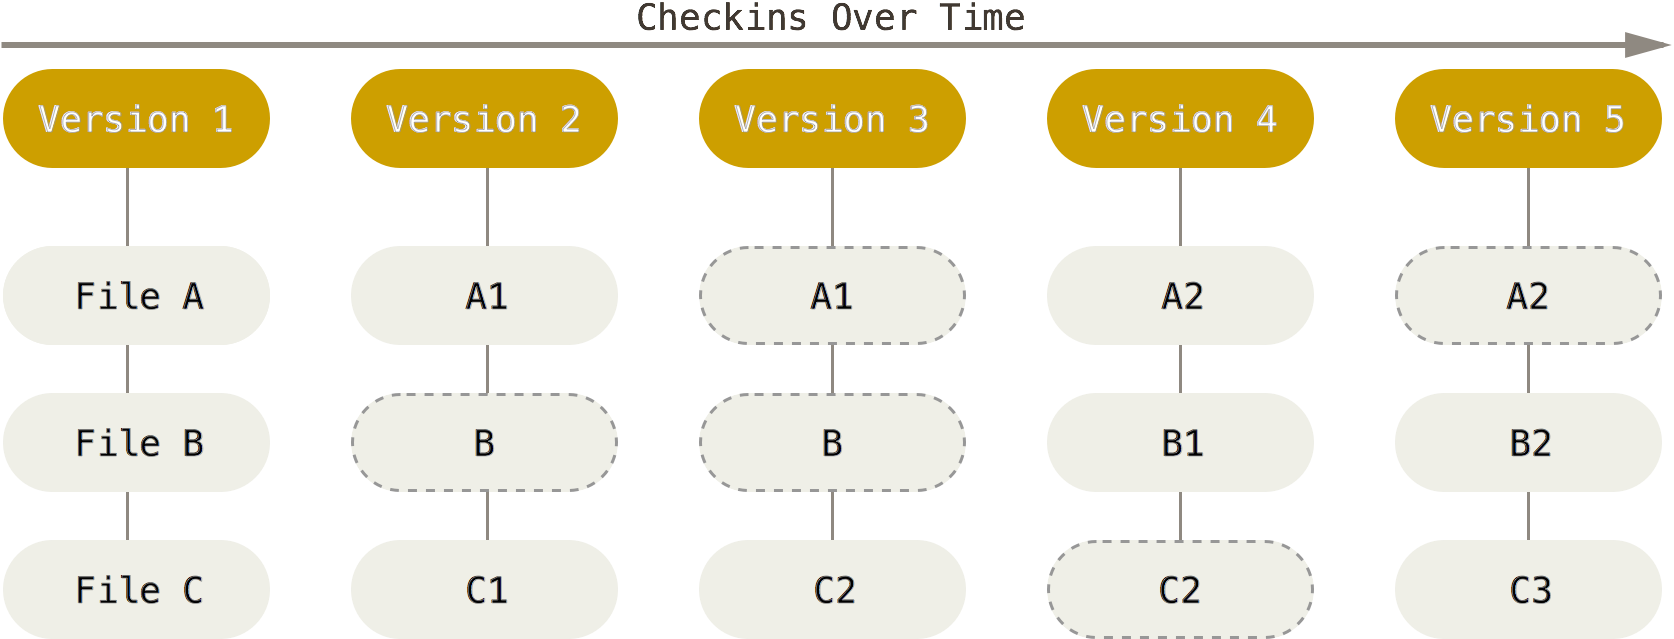
\includegraphics[width=0.8\textwidth]{images/snapshots}
		\end{center}
	\end{frame}


\section{What Does Using Git Look Like?}

	\begin{frame}
		\frametitle{Example Git History}
		\label{git_history_examples}
		Let me show you some example repositories
		\begin{itemize}
			\item \href{https://github.com/jamietanna/dotfiles-arch}{My dotfiles}
			\item {\color{red}\href{https://git.kernel.org}{The Linux Kernel}}
				\begin{itemize}
					\item i.e. \href{https://git.kernel.org/cgit/linux/kernel/git/tip/tip.git/log/}{\texttt{tip.git}}
				\end{itemize}

			\item \href{https://github.com/spring-projects/spring-boot}{\texttt{spring-boot}}
		\end{itemize}
	\end{frame}

	\begin{frame}
		\frametitle{Practical Demo}
		Note: this demo has been influenced by:
		\begin{itemize}
			\item \texttt{giteveryday(7)}
			\item \texttt{gitcore-tutorial(7)}
		\end{itemize}
	\end{frame}

	\begin{frame}
		\frametitle{Practical Demo}
		\begin{exampleblock}{Creating a Repository}
			We need to first create our repository:
			\begin{itemize}
 				\item \texttt{cd /path/to/folder}
 				\item \texttt{git init}
			\end{itemize}
		\end{exampleblock}
	\end{frame}

	\begin{frame}
		\frametitle{Practical Demo}
		\begin{exampleblock}{Create some files}
			\begin{itemize}
				\item \texttt{\$EDITOR helloworld.py}
				\item \texttt{\$EDITOR README.md}
				\item \texttt{git status}
				\item \footnotedef{Stage}{Add files to be \textbf{ready to be} committed} the files: \texttt{git add helloworld.py README.py}
				\item \texttt{git status}
			\end{itemize}
		\end{exampleblock}
		\begin{center}
			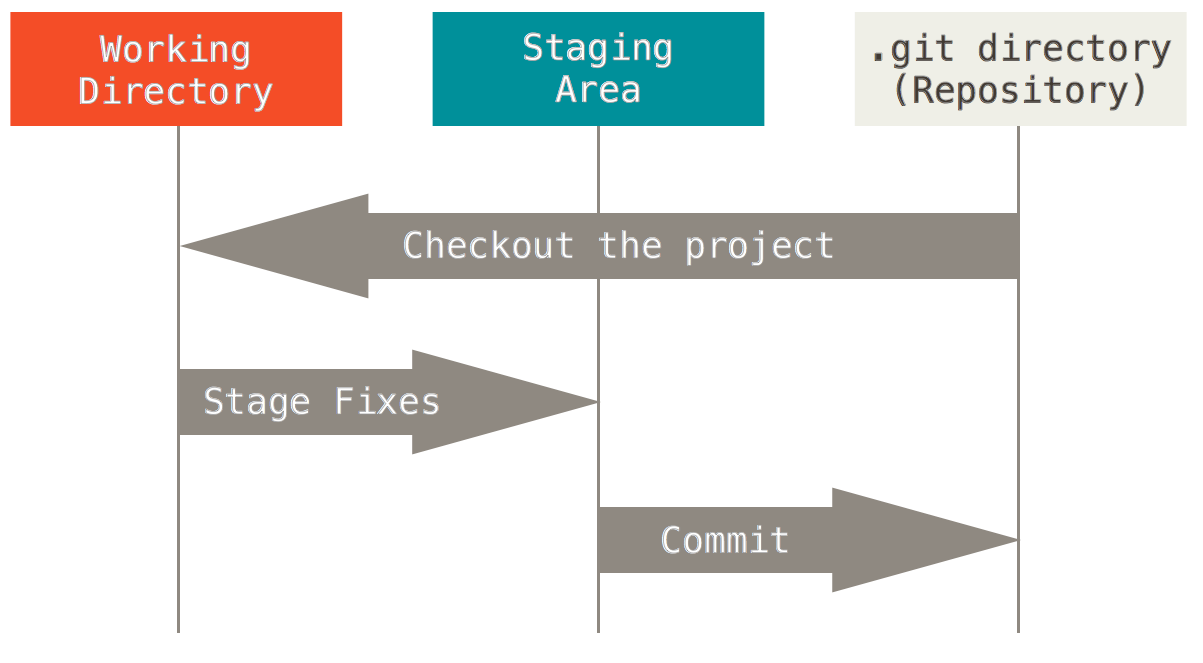
\includegraphics[width=0.6\textwidth]{images/areas.png}
		\end{center}
	\end{frame}

	\begin{frame}
		\frametitle{Practical Demo}
		\begin{exampleblock}{Committing}
			\begin{itemize}
				\item \texttt{git status}
				\item \texttt{git commit}
				\item \texttt{git status}
			\end{itemize}
		\end{exampleblock}
	\end{frame}
	\begin{frame}
		\frametitle{Writing Good Commit Messages}
		\begin{figure}
			\centering
			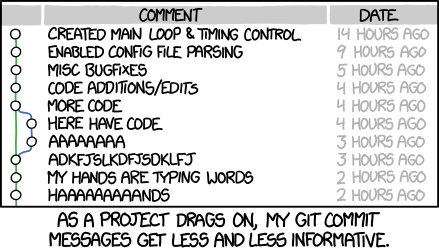
\includegraphics[width=0.9\textwidth]{./images/git_commit.png}
			\caption{Alt-text: \texttt{Merge branch 'asdfasjkfdlas/alkdjf' into sdkjfls-final}~\cite{XKCDGitCommit}}
		\end{figure}
	\end{frame}

	\begin{frame}
		\frametitle{Writing Good Commit Messages}

		\begin{itemize}
			\item Quickly skip back to slide \hyperlink{git_history_examples}{\ref{git_history_examples}}
			\item 50 chars - summary
			\item 72 chars wrapped - explanation
			\begin{itemize}
				\item Why have you added this change?
				\item What benefit/effect does it add to the repo?
				\item Does it solve any bugs/issues?
				\item Does it solve any bugs/issues?
				\item Explain \textbf{what and why}, not how
			\end{itemize}

			\item Bullet points
			\item Adapted from~\cite{ChrisBeamsGitCommit} and~\cite{GHErlangOTPWikiWGCM}
		\end{itemize}
	\end{frame}

	\begin{frame}
		\frametitle{Seeing What's Changed}
		\begin{exampleblock}{Making a few more changes}
			\begin{itemize}
				\item \texttt{\$EDITOR helloworld.py}
				\item \texttt{git status}
				\item Seeing what's changed: \texttt{git diff}
				\item \texttt{git add helloworld.py}
				\item \texttt{git diff} vs \texttt{git diff --cached}?
			\end{itemize}
		\end{exampleblock}
	\end{frame}

	\begin{frame}
		\frametitle{Unstaging Files}
		\begin{exampleblock}{``Oops, I didn't mean to add that file''}
			\begin{itemize}
				\item \texttt{\$EDITOR helloworld.py}
				\item \texttt{\$EDITOR README.md}
				\item \texttt{git status}
				\item \texttt{git add helloworld.py}
				\item \texttt{git reset}
			\end{itemize}
		\end{exampleblock}
	\end{frame}

	\begin{frame}
		\frametitle{Viewing History}
		\begin{exampleblock}{How can I see what I've done?}
			\begin{itemize}
				\item \texttt{git log}
				\item \texttt{git log --oneline}
				\item \texttt{git show \$SHA}
			\end{itemize}
		\end{exampleblock}
	\end{frame}

% Branching
	\begin{frame}
		\frametitle{Branching and Merging}
		\begin{exampleblock}{Branching and Merging}
			\begin{itemize}
				\item Imagine our current tree like so:
			\end{itemize}
		\end{exampleblock}

		\begin{center}
			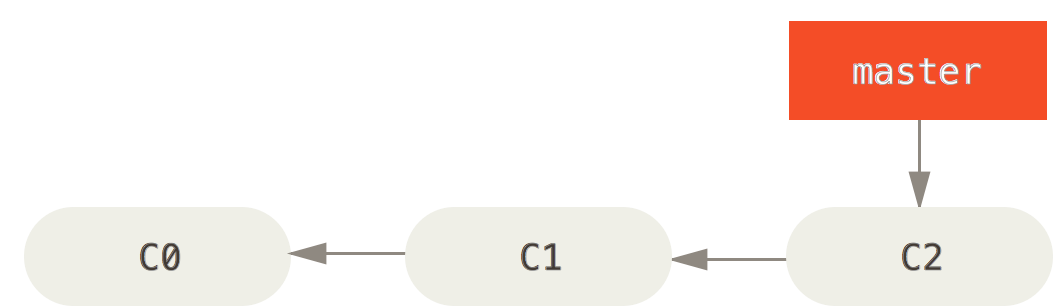
\includegraphics[width=0.7\textwidth]{./images/basic-branching-1.png}
		\end{center}
	\end{frame}

	\begin{frame}
		\frametitle{Branching and Merging}
		\begin{exampleblock}{Creating a Branch}
			\begin{itemize}
				\item \texttt{git branch}
				\item \texttt{git branch iss53}
				\item \texttt{git branch}
				\item \texttt{git checkout iss53}
				\item or: \texttt{git checkout -b iss53}
			\end{itemize}
		\end{exampleblock}

		\begin{center}
			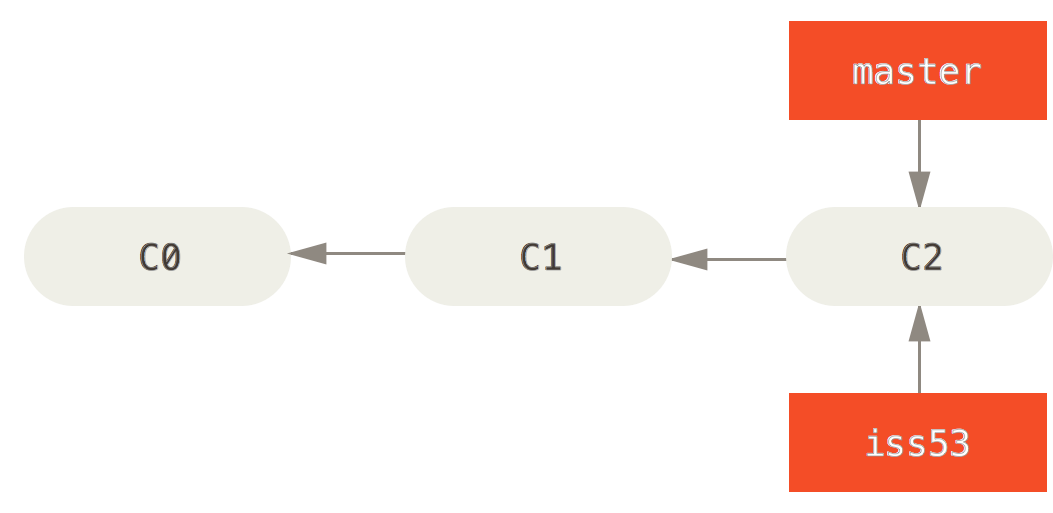
\includegraphics[width=0.7\textwidth]{./images/basic-branching-2.png}
		\end{center}
	\end{frame}

	\begin{frame}
		\frametitle{Branching and Merging}
		\begin{exampleblock}{Making a Change on a Branch}
			\begin{itemize}
				\item Now you need to make a fix on \texttt{iss53}:
				\item \texttt{\$EDITOR \$FILENAME}
				\item \texttt{git add \$FILENAME}
				\item \texttt{git commit}
			\end{itemize}
		\end{exampleblock}
		\begin{center}
			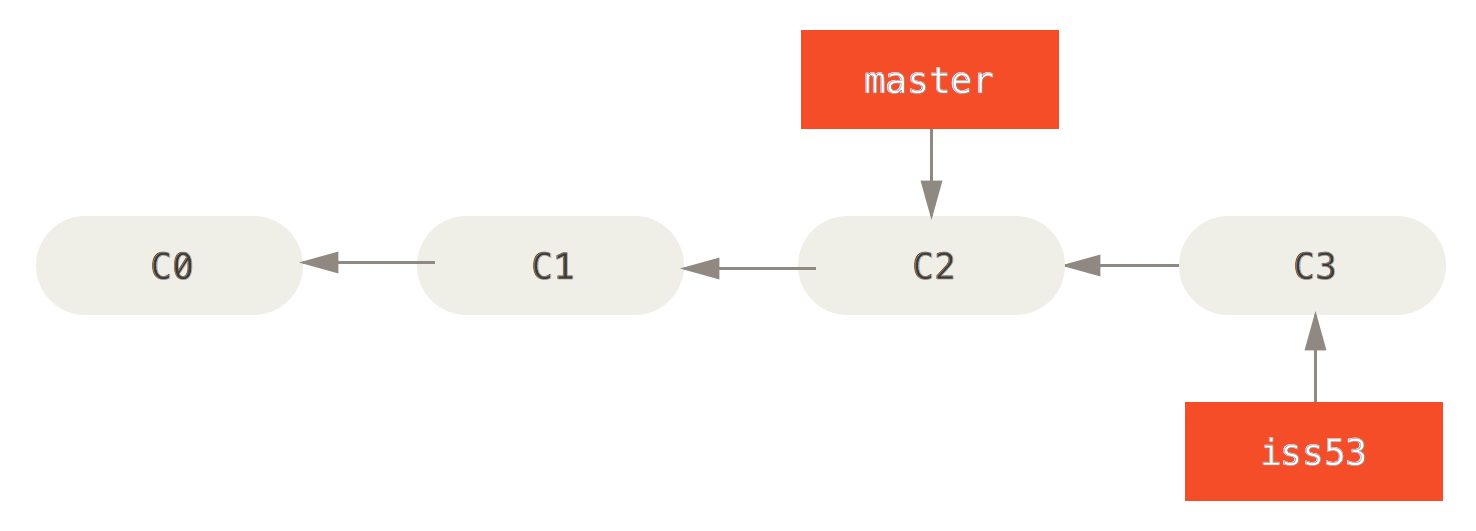
\includegraphics[width=0.8\textwidth]{./images/basic-branching-3.png}
		\end{center}
	\end{frame}

	\begin{frame}
		\frametitle{Branching and Merging}
		\begin{exampleblock}{Changing Another Branch}
			\begin{itemize}
				\item \texttt{git checkout master}
				\item \texttt{git checkout -b hotfix}
				\item \texttt{\$EDITOR \$FILENAME}
				\item \texttt{git add \$FILENAME}
				\item \texttt{git commit}
				\item \texttt{git log --graph}
			\end{itemize}
		\end{exampleblock}
		\begin{center}
			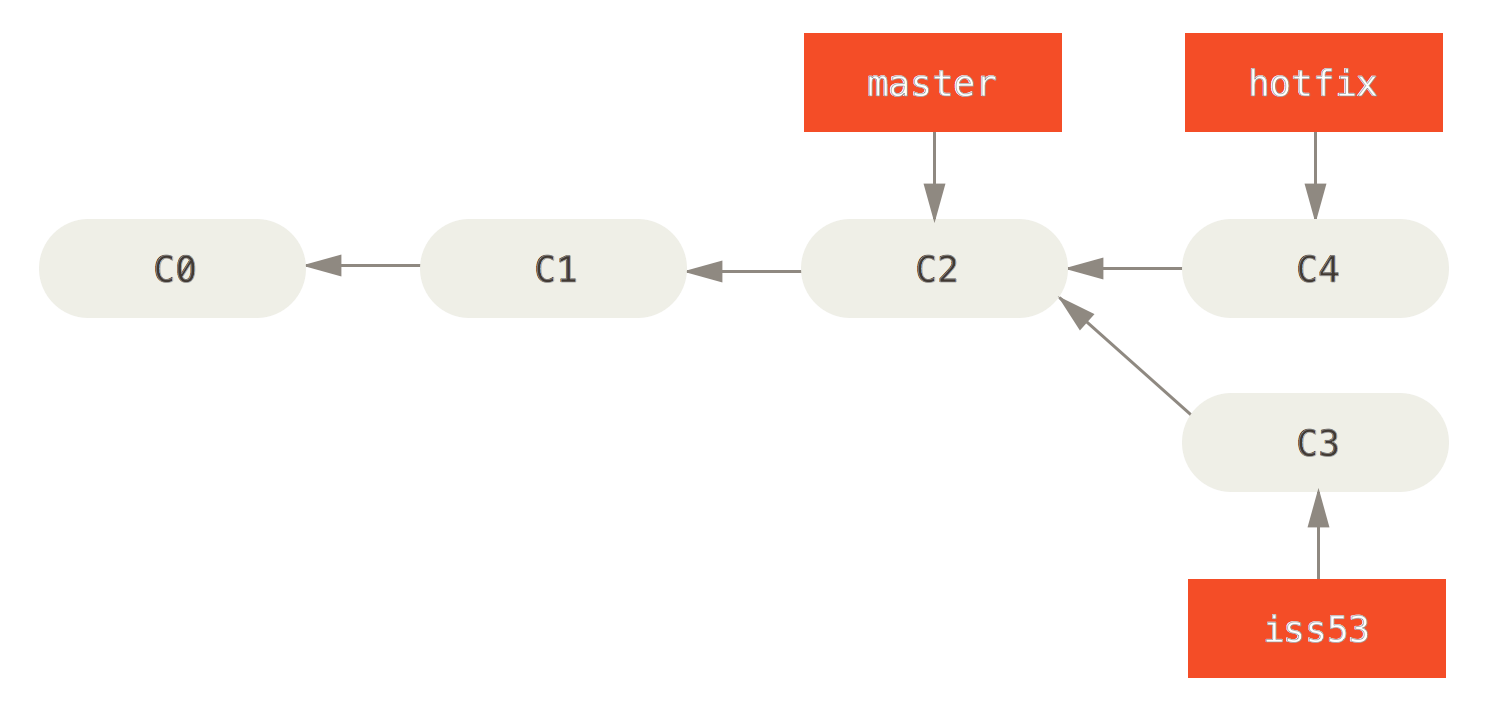
\includegraphics[width=0.65\textwidth]{./images/basic-branching-4.png}
		\end{center}
	\end{frame}

	\begin{frame}
		\frametitle{Branching and Merging}
		\begin{exampleblock}{Merging Branches}
			\begin{itemize}
				\item Then we need to merge the changes into master
				\item \texttt{git checkout master}
				\item \texttt{git merge hotfix}
			\end{itemize}
		\end{exampleblock}
		\begin{center}
			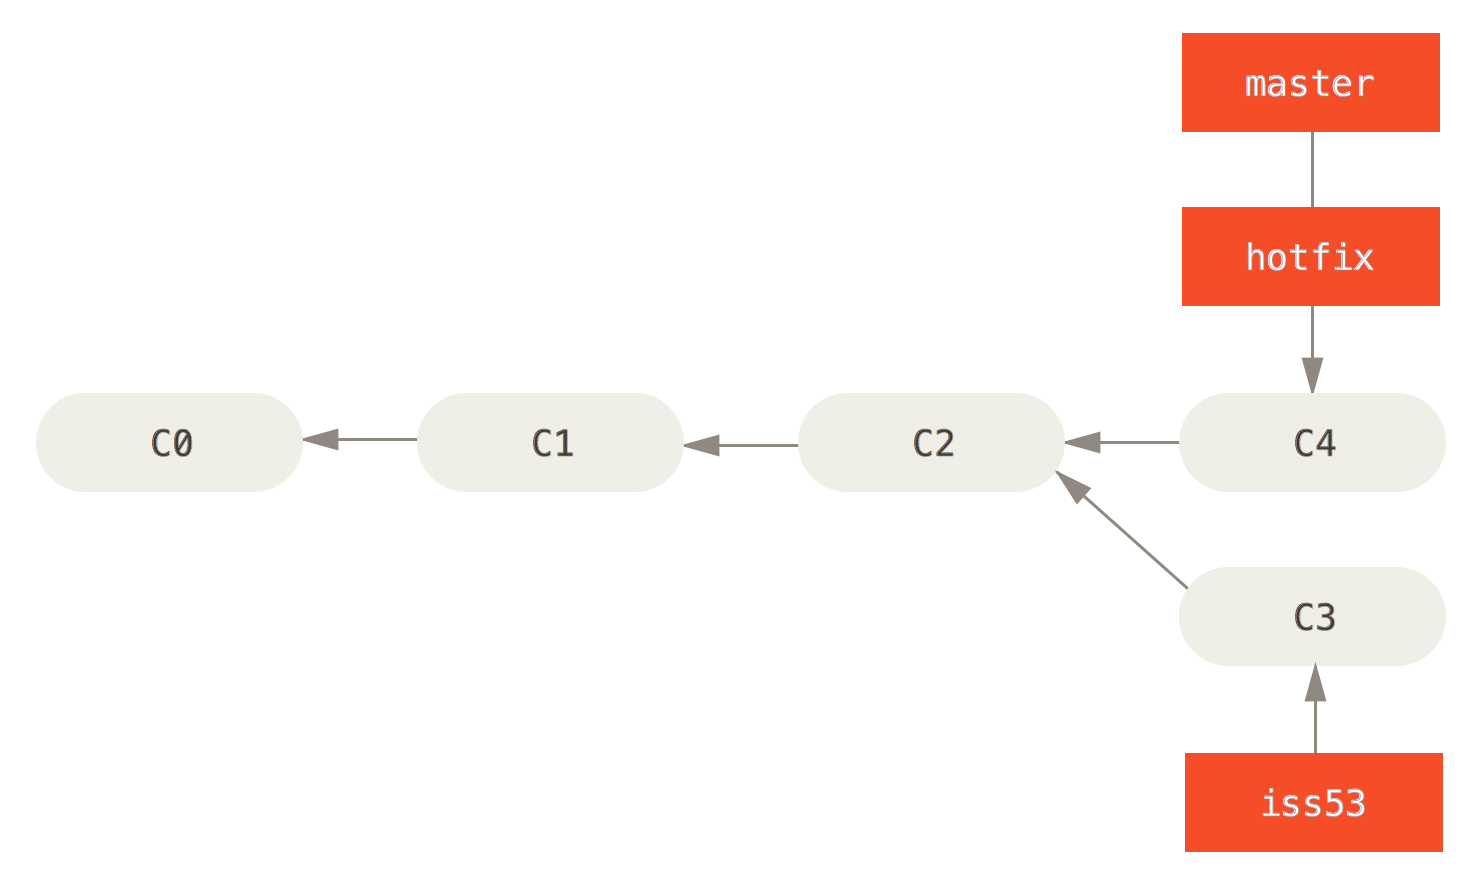
\includegraphics[width=0.7\textwidth]{./images/basic-branching-5.png}
		\end{center}
	\end{frame}

	\begin{frame}
		\frametitle{Branching and Merging}

		\begin{itemize}
			\item For a bit more in-depth example, I'd definitely recommend \url{http://git-scm.com/book/en/v2/Git-Branching-Branches-in-a-Nutshell} and \url{https://try.github.io/}
		\end{itemize}
	\end{frame}

%</Branching>
	\begin{frame}
		\frametitle{Working With Remotes}
		\begin{exampleblock}{Working on other projects}
			\begin{itemize}
				\item \texttt{git clone \$URL}
				\item \texttt{git pull}
				\item \texttt{git remote}
			\end{itemize}
		\end{exampleblock}
	\end{frame}

\label{hosted_vcs_compare}
\section{Github and Other Git Hosting}

\begin{frame}
	\frametitle{Why Would I Want Hosted Git Repos?}
	\begin{itemize}
		\item Why would you want to host it?
		\item Didn't I say centralised was a bad idea though?
		\item Backup against device crash, inaccessibility
		\item Collaboration
		\item Convenience
	\end{itemize}
\end{frame}

\begin{frame}
	\AddToShipoutPictureFG*{\includegraphics[width=\paperwidth]{backgrounds/github.pdf}}
	\frametitle{Github}

	\begin{itemize}
		\item \url{https://www.github.com}
		\item Github is \emph{one of} the most popular repository hosting site that is
		\item Unlimited public, paid private repos
	\end{itemize}
\end{frame}

\begin{frame}
	\frametitle{GitLab}
	\AddToShipoutPictureFG*{\includegraphics[width=\paperwidth]{backgrounds/gitlab.pdf}}

	\begin{itemize}
		\item \url{https://www.gitlab.com}
		\item Up and coming to become really great Git hosting
		\item My new hosting for new projects
		\item Integrated Continuous Integration (see next week's talk!)
		\item Unlimited public + private repos
	\end{itemize}
\end{frame}

\begin{frame}
	\AddToShipoutPictureFG*{\includegraphics[width=\paperwidth]{backgrounds/bitbucket.pdf}}
	\frametitle{BitBucket}

	\begin{itemize}
		\item \url{https://bitbucket.org}
		\item Previously for private, now use GitLab
		\item Unlimited public + private repos
	\end{itemize}
\end{frame}

\section{Conclusion}

\begin{frame}{Summary}

	Get the source of this presentation at

	\begin{center}\url{https://github.com/jamietanna/gittalk15}\end{center}

	For further reading, check out the incredibly awesome (and free) \href{http://git-scm.com/book/en/v2}{Git Book}.

	This presentation is licensed under a
	\href{http://creativecommons.org/licenses/by-sa/4.0/}{Creative Commons
	Attribution-ShareAlike 4.0 International License}.

	\begin{center}\ccbysa\end{center}

\end{frame}

% \plain{Questions?}

\begin{frame}[allowframebreaks]

	\frametitle{References}

	\bibliography{./intro-to-git.bib}
	\bibliographystyle{abbrv}

\end{frame}

\end{document}
